% Copyright 2010 by Frank Wood

\documentclass[xcolor=dvipsnames]{beamer}
\usepackage{algorithm}
\usepackage{algorithmic}
\usepackage{subfigure}
\usepackage[]{natbib}
%\usepackage{amsmath,amssymb,graphicx,subfig}

% Setup appearance:

\usetheme{Madrid}
%\usetheme{Copenhagen}
\usefonttheme[onlylarge]{structurebold}
\usecolortheme[RGB={0,63,135}]{structure} 
\setbeamerfont*{frametitle}{size=\normalsize,series=\bfseries}
%\setbeamertemplate{navigation symbols}{}

% Standard packages

\usepackage[english]{babel}
%\usepackage[latin1]{inputenc}
%\usepackage{times}
%\usepackage[T1]{fontenc}
%\usepackage{nnfootnote}
\usepackage{amsfonts}
\usepackage{amsmath}
\usepackage{xspace}

%\newcommand{\argmax}{\operatornamewithlimits{argmax}}
\def\newblock{\hskip .11em plus .33em minus .07em}
% Setup TikZ

%\usepackage{tikz}
%\usetikzlibrary{arrows}
%\tikzstyle{block}=[draw opacity=0.7,line width=1.4cm]



\defcitealias{Huggins-2012-AISTATS}{Huggins and W, 2011}
\defcitealias{Dewar:2011}{Dewar, Wiggins and W, 2011}


\newcommand{\eq}{\begin{equation*}}
\newcommand{\en}{\end{equation*}}
\newcommand{\eqa}{\begin{eqnarray*}}
\newcommand{\ena}{\end{eqnarray*}}
\newcommand{\eqn}{\begin{equation}}
\newcommand{\enn}{\end{equation}}
\newcommand{\eqan}{\begin{eqnarray}}
\newcommand{\enan}{\end{eqnarray}}
\newcommand{\GP}{$\Gamma$P}
\newcommand{\bsym}{\boldsymbol}

% Author, Title, etc.

\title[EDHMM Inference] 
{
  Inference in Explicit Duration \\
  Hidden Markov Models %\\ \small{~}\\ 
 % \tiny{How I Learned to Stop Worrying and Love the Infinite}
   % \tiny{A novel, general construction }
}

\author[Wood]
{
  Frank~Wood\\
  ~\\%\inst{1}\\
  \tiny{Joint work with Chris Wiggins, Mike Dewar}
}

\institute[Columbia University]
{
  %\inst{1}%
  Columbia University
}

\date[November, 2011]
{November, 2011}

%\def\blfootnote{\xdef\@thefnmark{}\@footnotetext}


% The main document
% !TEX root = talk.tex

\newcommand{\comment}[1]{}
%\newcommand{\comment}[1]{{\marginpar{\tiny {#1} }}}
\def\todo#1{TODO(#1)}

\def\bigO{{\mathcal O}}
\def\balpha{\mbox{\boldmath $\alpha$}}
\def\bbeta{\mbox{\boldmath $\beta$}}
\def\beeta{\mbox{\boldmath $\eta$}}
\def\blambda{\mbox{\boldmath $\lambda$}}
\def\bmu{\mbox{\boldmath $\mu$}}
\def\bphi{\mbox{\boldmath $\phi$}}
\def\bpsi{\mbox{\boldmath $\psi$}}
\def\bsigma{\mbox{\boldmath $\sigma$}}
\def\btau{\mbox{\boldmath $\tau$}}
\def\btheta{\mbox{\boldmath $\theta$}}
\def\dbphi{\dot{\mbox{\boldmath $\phi$}}}
\def\dbtau{\dot{\mbox{\boldmath $\tau$}}}
\def\dbtheta{\dot{\mbox{\boldmath $\theta$}}}

%\newcommand{\nofootnotemark}{\let\@makefnmark\relax}
\newcommand{\bX}{\mathbf{X}}
\newcommand{\bY}{\mathbf{Y}}
\newcommand{\bW}{\mathbf{W}}
\newcommand{\bZ}{\mathbf{Z}}
\newcommand{\bH}{\mathbf{H}}
\newcommand{\bQ}{\mathbf{Q}}
\newcommand{\bA}{\mathbf{A}}
\newcommand{\bI}{\mathbf{I}}
\newcommand{\by}{\mathbf{y}}
\newcommand{\bz}{\mathbf{z}}
\newcommand{\bx}{\mathbf{x}}

\newcommand{\ith}{i^\mathrm{th}}
\def\A{{\bf A}}
\def\B{{\bf B}}
\def\C{{\bf C}}
\def\D{{\bf D}}
\def\F{{\bf F}}
\def\L{{\bf L}}
\def\M{{\bf M}}
\def\W{{\bf W}}
\def\I{{\bf I}}
\def\J{{\bf J}}
\def\R{{\bf R}}
\def\U{{\bf U}}
\def\V{{\bf V}}
\def\b{{\bf b}}
\def\c{{\bf c}}
\def\d{{\bf d}}
\def\r{{\bf r}}
\def\s{{\bf s}}
\def\t{{\bf t}}
\def\u{{\bf u}}
\def\v{{\bf v}}
\def\f{{\bf f}}
\def\x{{\bf x}}
\def\y{{\bf y}}
\def\w{{\bf w}}
\def\vo{{\bf o}}
\def\p{{\bf p}}
\def\O{{\bf 0}}
%\def\a{{\bf a}}


\def\vbpsi{\vec{\mbox{\boldmath $\psi$}}} 
\def\vpsi{\vec{\psi}} 
\def\vbphi{\vec{\mbox{\boldmath $\phi$}}} 
\def\vphi{\vec{\phi}} 
\def\vbtau{\vec{\mbox{\boldmath $\tau$}}} 
\def\vbtheta{\vec{\mbox{\boldmath $\theta$}}} 
\def\vD{\vec{D}}
\def\vf{\vec{\bf f}}
\def\vF{\vec{\bf F}}
\def\vI{\vec{\bf I}}
\def\vR{\vec{\bf R}}
\def\vv{\vec{v}}
\def\vV{\vec{\bf V}}

\def\pon{p_{\mathrm{on}}}
\def\poff{p_{\mathrm{off}}}

\def\tr{^{\text{T}}}

%%% Vector notation for sections 3 and 4
%%% Vector notation for sections 3 and 4
\def\mvec{\vec{m}}
\def\fvec{\vec{f}}
\def\appfvec{\vec{f}_k}
\def\avec{\vec{a}}
\def\bvec{\vec{b}}
\def\evec{\vec{e}}
\def\uvec{\vec{u}}
\def\xvec{\vec{x}}
\def\wvec{\vec{w}}
\def\gradvec{\vec{\nabla}}

\def\aM{\mbox{\bf a}_M}
\def\aS{\mbox{\bf a}_S}
\def\aO{\mbox{\bf a}_O}
\def\aL{\mbox{\bf a}_L}
\def\aP{\mbox{\bf a}_P}
\def\ai{\mbox{\bf a}_i}
\def\aj{\mbox{\bf a}_j}
\def\an{\mbox{\bf a}_n}
\def\a1{\mbox{\bf a}_1}
\def\a2{\mbox{\bf a}_2}
\def\a3{\mbox{\bf a}_3}
\def\a4{\mbox{\bf a}_4}

%\def\x{\mbox{\bf x\/}}
%\def\X{\mbox{\bf X}}
%\def\A{\mbox{\bf A}}
%\def\P{\mbox{\bf P}}
%\def\C{\mbox{\bf C}}
%\def\c{\mbox{\bf c}}
%\def\b{\mbox{\bf b}}
%\def\o{\mbox{\bf o}}
%\def\h{\mbox{\bf h}}
%\def\f{\mbox{\bf f}}
%\def\x{\mbox{\bf x}}
%\def\sx{\mbox{\scriptsize\bf x}}
%\def\z{\mbox{\bf z}}
%\def\l{\mbox{\bf l}}
%\def\m{\mbox{\bf m}}
%\def\bi{\mbox{\bf i}}
%\def\u{\mbox{\bf u}}
%\def\v{\mbox{\bf v}}
\def\a{\mbox{\bf a}}
%\def\p{\mbox{\bf p}}
%\def\r{\mbox{\bf r}}
%\def\d{\mbox{\bf d}}
%\def\Q{\mbox{\bf Q}}
%\def\s{\mbox{\bf s}}
%\def\st{\mbox{\scriptsize\bf t}}
%\def\ss{\mbox{\scriptsize\bf s}}
%\def\t{\mbox{\bf t}}
%\def\cR{{\cal R}}
%\def\calD{{\cal D}}
%\def\calS{{\cal S}}
%\def\g{\mbox{\bf g}}
%\def\e{\mbox{\bf e}}
%\def\flow{\{\mbox{\bf u}\}}
%\def\appearChange{iconic change}

\def\sigmae{\sigma}
\def\sigmam{\sigma}

\newcommand{\eg}{e.\thinspace{}g.,\@\xspace}
\newcommand{\egn}{e.\thinspace{}g.\@\xspace}
\newcommand{\cf}{cf.\@\xspace}
\newcommand{\ie}{i.\thinspace{}e.,\@\xspace}
\newcommand{\ien}{i.\thinspace{}e.\@\xspace}
\newcommand{\iid}{i.\thinspace{}i.\thinspace{}d.\@\xspace}


%\newcommand{\comment}[1]{}
\newcommand{\ponedec}{\mathcal{P}^\downarrow_1}
\newcommand{\pone}{\mathcal{P}_1}
\newcommand{\rank}[1]{\mathrm{RANK}\left[#1\right]}
\newcommand{\E}[1]{\mathrm{E}\left[#1\right]}
%\newcommand{\PY}{\mathcal{PY}}
%\newcommand{\DP}{\mathcal{DP}}
%\newcommand{\iid}{iid.}
\newcommand{\drawiid}{\stackrel{\text{iid}}{\sim}}
\newcommand{\vect}[1]{\mathbf{#1}}
\newcommand{\indicator}[1]{\text{I}\left[ #1 \right]}
\newcommand{\pdcoag}{PD(d_1,0)-\text{COAG}}
%\newcommand{\todo}{\textbf{*TODO*}}
\newcommand{\igram}{\text{$\infty$-gram}}
\newcommand{\Prob}{\text{P}}

\def\mm{sequence memoizer }
\def\MM{SM }

\def\pibf{{\boldsymbol{\pi}}}
\def\kapbf{\boldsymbol{\kappa}}
\def\taubf{\boldsymbol{\tau}}
\def\thebf{\boldsymbol{\theta}}
\def\rhobf{\boldsymbol{\rho}}
\def\phibf{\boldsymbol{\phi}}
\def\pbf{\mathbf{p}}
\def\qbf{\mathbf{q}}
\def\sbf{\mathbf{s}}
\def\tbf{\mathbf{t}}
\def\ybf{\mathbf{y}}
\def\ubf{\mathbf{u}}
\def\Ave{\mathbb{E}}

\def\wbf{\mathbf{w}}
\def\xbf{\mathbf{x}}
\def\rbf{\mathbf{r}}
\def\tbf{\mathbf{t}}
\def\kbf{\mathbf{k}}
\def\Xbf{\mathbf{X}}
\def\0bf{\mathbf{0}}
\def\Ibf{\mathbf{I}}
\def\phibf{\mathbf{\phi}}
\def\Phibf{\mathbf{\Phi}}
\def\disteq{{\stackrel{D}{=}}}
\def\EE{{\mathbb{E}}}
\def\GG{\mathcal{G}}
\def\G{G}
\def\U{U}

\def\phiv{\varphi}
\def\phivbf{\boldsymbol{\varphi}}

\def\Ocal{\mathcal{O}}
\DeclareMathOperator*{\Var}{Var}

\DeclareMathOperator*{\Bet}{Beta}
\DeclareMathOperator{\coag}{COAG}
\DeclareMathOperator{\frag}{FRAG}
\DeclareMathOperator*{\rnk}{RANK}
\DeclareMathOperator*{\gem}{GEM}
\DeclareMathOperator*{\pd}{PD}
\DeclareMathOperator*{\py}{PY}
\DeclareMathOperator*{\DP}{DP}
\DeclareMathOperator*{\PY}{PY}
\DeclareMathOperator*{\gd}{GDir}
\DeclareMathOperator*{\Dir}{Dir}
\DeclareMathOperator*{\CRP}{CRP}
\DeclareMathOperator*{\argmax}{argmax}



%%% Local Variables: 
%%% mode: latex
%%% TeX-master: "paper"
%%% End: 
% !TEX root = talk.tex
%
%\newcommand{\comment}[1]{}
%%\newcommand{\comment}[1]{{\marginpar{\tiny {#1} }}}
%
%\def\bigO{{\mathcal O}}
%\def\balpha{\mbox{\boldmath $\alpha$}}
%\def\bbeta{\mbox{\boldmath $\beta$}}
%\def\beeta{\mbox{\boldmath $\eta$}}
%\def\blambda{\mbox{\boldmath $\lambda$}}
%\def\bmu{\mbox{\boldmath $\mu$}}
%\def\bphi{\mbox{\boldmath $\phi$}}
%\def\bpsi{\mbox{\boldmath $\psi$}}
%\def\bsigma{\mbox{\boldmath $\sigma$}}
%\def\btau{\mbox{\boldmath $\tau$}}
%\def\btheta{\mbox{\boldmath $\theta$}}
%\def\dbphi{\dot{\mbox{\boldmath $\phi$}}}
%\def\dbtau{\dot{\mbox{\boldmath $\tau$}}}
%\def\dbtheta{\dot{\mbox{\boldmath $\theta$}}}
%
%%\newcommand{\nofootnotemark}{\let\@makefnmark\relax}
%\newcommand{\bX}{\mathbf{X}}
%\newcommand{\bY}{\mathbf{Y}}
%\newcommand{\bW}{\mathbf{W}}
%\newcommand{\bZ}{\mathbf{Z}}
%\newcommand{\bH}{\mathbf{H}}
%\newcommand{\bQ}{\mathbf{Q}}
%\newcommand{\bA}{\mathbf{A}}
%\newcommand{\bI}{\mathbf{I}}
%\newcommand{\by}{\mathbf{y}}
%\newcommand{\bz}{\mathbf{z}}
%\newcommand{\bx}{\mathbf{x}}
%
%\newcommand{\ith}{i^\mathrm{th}}
%\def\A{{\bf A}}
%\def\B{{\bf B}}
%\def\C{{\bf C}}
%\def\D{{\bf D}}
%\def\F{{\bf F}}
%\def\L{{\bf L}}
%\def\M{{\bf M}}
%\def\W{{\bf W}}
%\def\I{{\bf I}}
%\def\J{{\bf J}}
%\def\R{{\bf R}}
%\def\U{{\bf U}}
%\def\V{{\bf V}}
%\def\b{{\bf b}}
%\def\c{{\bf c}}
%\def\d{{\bf d}}
%\def\r{{\bf r}}
%\def\s{{\bf s}}
%\def\t{{\bf t}}
%\def\u{{\bf u}}
%\def\v{{\bf v}}
%\def\f{{\bf f}}
%\def\x{{\bf x}}
%\def\y{{\bf y}}
%\def\w{{\bf w}}
%\def\vo{{\bf o}}
%\def\p{{\bf p}}
%\def\O{{\bf 0}}
%%\def\a{{\bf a}}
%
%
%\def\vbpsi{\vec{\mbox{\boldmath $\psi$}}} 
%\def\vpsi{\vec{\psi}} 
%\def\vbphi{\vec{\mbox{\boldmath $\phi$}}} 
%\def\vphi{\vec{\phi}} 
%\def\vbtau{\vec{\mbox{\boldmath $\tau$}}} 
%\def\vbtheta{\vec{\mbox{\boldmath $\theta$}}} 
%\def\vD{\vec{D}}
%\def\vf{\vec{\bf f}}
%\def\vF{\vec{\bf F}}
%\def\vI{\vec{\bf I}}
%\def\vR{\vec{\bf R}}
%\def\vv{\vec{v}}
%\def\vV{\vec{\bf V}}
%
%\def\pon{p_{\mathrm{on}}}
%\def\poff{p_{\mathrm{off}}}
%
%\def\tr{^{\text{T}}}
%
%%%% Vector notation for sections 3 and 4
%%%% Vector notation for sections 3 and 4
%\def\mvec{\vec{m}}
%\def\fvec{\vec{f}}
%\def\appfvec{\vec{f}_k}
%\def\avec{\vec{a}}
%\def\bvec{\vec{b}}
%\def\evec{\vec{e}}
%\def\uvec{\vec{u}}
%\def\xvec{\vec{x}}
%\def\wvec{\vec{w}}
%\def\gradvec{\vec{\nabla}}
%
%\def\aM{\mbox{\bf a}_M}
%\def\aS{\mbox{\bf a}_S}
%\def\aO{\mbox{\bf a}_O}
%\def\aL{\mbox{\bf a}_L}
%\def\aP{\mbox{\bf a}_P}
%\def\ai{\mbox{\bf a}_i}
%\def\aj{\mbox{\bf a}_j}
%\def\an{\mbox{\bf a}_n}
%\def\a1{\mbox{\bf a}_1}
%\def\a2{\mbox{\bf a}_2}
%\def\a3{\mbox{\bf a}_3}
%\def\a4{\mbox{\bf a}_4}
%
%%\def\x{\mbox{\bf x\/}}
%%\def\X{\mbox{\bf X}}
%%\def\A{\mbox{\bf A}}
%%\def\P{\mbox{\bf P}}
%%\def\C{\mbox{\bf C}}
%%\def\c{\mbox{\bf c}}
%%\def\b{\mbox{\bf b}}
%%\def\o{\mbox{\bf o}}
%%\def\h{\mbox{\bf h}}
%%\def\f{\mbox{\bf f}}
%%\def\x{\mbox{\bf x}}
%%\def\sx{\mbox{\scriptsize\bf x}}
%%\def\z{\mbox{\bf z}}
%%\def\l{\mbox{\bf l}}
%%\def\m{\mbox{\bf m}}
%%\def\bi{\mbox{\bf i}}
%%\def\u{\mbox{\bf u}}
%%\def\v{\mbox{\bf v}}
%\def\a{\mbox{\bf a}}
%%\def\p{\mbox{\bf p}}
%%\def\r{\mbox{\bf r}}
%%\def\d{\mbox{\bf d}}
%%\def\Q{\mbox{\bf Q}}
%%\def\s{\mbox{\bf s}}
%%\def\st{\mbox{\scriptsize\bf t}}
%%\def\ss{\mbox{\scriptsize\bf s}}
%%\def\t{\mbox{\bf t}}
%%\def\cR{{\cal R}}
%%\def\calD{{\cal D}}
%%\def\calS{{\cal S}}
%%\def\g{\mbox{\bf g}}
%%\def\e{\mbox{\bf e}}
%%\def\flow{\{\mbox{\bf u}\}}
%%\def\appearChange{iconic change}
%
%\def\sigmae{\sigma}
%\def\sigmam{\sigma}
%
%\newcommand{\eg}{e.\thinspace{}g.,\@\xspace}
%\newcommand{\egn}{e.\thinspace{}g.\@\xspace}
%\newcommand{\cf}{cf.\@\xspace}
%\newcommand{\ie}{i.\thinspace{}e.,\@\xspace}
%\newcommand{\ien}{i.\thinspace{}e.\@\xspace}
%\newcommand{\iid}{i.\thinspace{}i.\thinspace{}d.\@\xspace}
%
%
%%\newcommand{\comment}[1]{}
%\newcommand{\ponedec}{\mathcal{P}^\downarrow_1}
%\newcommand{\pone}{\mathcal{P}_1}
%\newcommand{\rank}[1]{\mathrm{RANK}\left[#1\right]}
%%\newcommand{\E}[1]{\mathrm{E}\left[#1\right]}
%%\newcommand{\PY}{\mathcal{PY}}
%%\newcommand{\DP}{\mathcal{DP}}
%%\newcommand{\iid}{iid.}
%\newcommand{\drawiid}{\stackrel{\text{iid}}{\sim}}
%\newcommand{\vect}[1]{\mathbf{#1}}
%\newcommand{\indicator}[1]{\text{I}\left[ #1 \right]}
%\newcommand{\pdcoag}{PD(d_1,0)-\text{COAG}}
%%\newcommand{\todo}{\textbf{*TODO*}}
%\newcommand{\igram}{\text{$\infty$-gram}}
%\newcommand{\Prob}{\text{P}}
%
%\def\mm{sequence memoizer }
%\def\MM{SM }
%
%\def\pibf{{\boldsymbol{\pi}}}
%\def\kapbf{\boldsymbol{\kappa}}
%\def\taubf{\boldsymbol{\tau}}
%\def\thebf{\boldsymbol{\theta}}
%\def\rhobf{\boldsymbol{\rho}}
%\def\phibf{\boldsymbol{\phi}}
%\def\pbf{\mathbf{p}}
%\def\qbf{\mathbf{q}}
%\def\sbf{\mathbf{s}}
%\def\tbf{\mathbf{t}}
%\def\ybf{\mathbf{y}}
%\def\ubf{\mathbf{u}}
%\def\Ave{\mathbb{E}}
%
%\def\wbf{\mathbf{w}}
%\def\xbf{\mathbf{x}}
%\def\rbf{\mathbf{r}}
%\def\tbf{\mathbf{t}}
%\def\kbf{\mathbf{k}}
%\def\Xbf{\mathbf{X}}
%\def\0bf{\mathbf{0}}
%\def\Ibf{\mathbf{I}}
%\def\phibf{\mathbf{\phi}}
%\def\Phibf{\mathbf{\Phi}}
%\def\disteq{{\stackrel{D}{=}}}
%\def\GG{\mathcal{G}}
%\def\G{G}
%\def\U{U}
%
%\def\phiv{\varphi}
%\def\phivbf{\boldsymbol{\varphi}}
%
%\def\Ocal{\mathcal{O}}
%\DeclareMathOperator*{\Var}{Var}
%
%\DeclareMathOperator*{\Bet}{Beta}
%\DeclareMathOperator{\coag}{COAG}
%\DeclareMathOperator{\frag}{FRAG}
%\DeclareMathOperator*{\rnk}{RANK}
%\DeclareMathOperator*{\gem}{GEM}
%\DeclareMathOperator*{\pd}{PD}
%\DeclareMathOperator*{\py}{PY}
%\DeclareMathOperator*{\DP}{DP}
%\DeclareMathOperator*{\PY}{PY}
%\DeclareMathOperator*{\gd}{GDir}
%\DeclareMathOperator*{\Dir}{Dir}
%\DeclareMathOperator*{\CRP}{CRP}
%\DeclareMathOperator*{\argmax}{argmax}
%
\def\GG{\mathcal{G}}
\def\data{\mathbf{x}}
%\def\EE{\mathbb{E}}
\def\disc{d}
%\newcommand{\delete}[1]{} %\textcolor{red}{#1}
%\newcommand{\rewrite}[1]{#1}%{\textcolor{blue}{#1}} %
%\newcommand{\lambdabf}{\boldsymbol{\lambda}}
%\newcommand{\vbf}{\mathbf{v}}
%\newcommand{\Psmooth}{\Prob_\text{smooth}}
%%\newcommand{\parent}{\pi}
%\newcommand{\suffix}{\sigma}
%\newcommand{\UHPYP}{SM}
%\newcommand{\PLUMP}{PLUMP}
%\newcommand{\Oh}{\mathcal{O}}
%\newcommand{\tree}{\mathcal{T}}
\newcommand{\cct}{\hat{\mathcal{T}}}
\newcommand{\cctx}{\cct(\data)}
\newcommand{\Gu}{G_{\ubf}}
%\newcommand{\GuSet}{\{G_{\ubf}\}_{\ubf \in \Sigma^*}}
%\newcommand{\E}{\mathrm{E}}
%\newcommand{\UpdatePath}{\text{\textsc{UpdatePath}}}
%\newcommand{\Path}{\ensuremath{(\ubf_0,\ldots,\ubf_P)}}
%\newcommand{\PathProbability}{\text{\textsc{PathProbability}}}
%\newcommand{\TT}{\mathcal{T}}
%\newcommand{\ral}[1]{\stackrel{\mathtt{#1}}{\rightarrow}}
\def\parent{{\sigma(\mathbf{u})}}
%
%%\def\newblock{\hskip .11em plus .33em minus .07em}
%
%
%% \newcommand{\cusk}{c_{\ubf s k}}
%% \newcommand{\cus}{c_{\ubf s \cdot}}
%% \newcommand{\cu}{c_{\ubf \cdot \cdot}}
%% \newcommand{\tus}{t_{\ubf s}}
%% \newcommand{\tu}{t_{\ubf \cdot}}
%\newcommand{\cusk}{c_{\ubf s k}}
%\newcommand{\cus}{c_{\ubf s}}
%\newcommand{\cu}{c_{\ubf \cdot}}
%\newcommand{\tus}{t_{\ubf s}}
%\newcommand{\tu}{t_{\ubf \cdot}}
%\newcommand{\cset}{\{\cusk\}_{s\in \Sigma,k \in \{1,\ldots,t_{\ubf s}\}}}
%\newcommand{\tset}{\{\tus\}_{s\in \Sigma}}
%\newcommand{\bydef}{\equiv}
%\newcommand{\state}{\mathcal{S}_{\xbf}}
%\newcommand{\statei}{\mathcal{S}_{\xbf_{1:i}}}
%%\newcommand{\emptystring}{\varepsilon}
%\newcommand{\gcount}{\hat{c}}
%\newcommand{\escape}{\mathtt{esc}}
%\def\prob{G}
%
%
%\newcommand{\todo}[1]{\begin{center}\textbf{TODO: } #1 \end{center}}
%\newcommand{\figref}[1]{\figurename~\ref{#1}}
%\newcommand{\predictive}{\Prob(x_i|\xbf_{1:i-1})}
%\newcommand{\ywcomment}[1]{\textbf{#1}}
%\newcommand{\jgcomment}[1]{ { \textcolor{red}{#1} } }
%
%\newcommand{\secref}[1]{Section \ref{#1}}
%
\def\context{\mathbf{u}}

%%% Local Variables: 
%%% mode: latex
%%% TeX-master: "paper"
%%% End: 


\usebackgroundtemplate{
\includegraphics[width=\paperwidth]{../columbia_background.png}}

\begin{document}

%\nofootnotemark
\begin{frame}
  \titlepage
\end{frame}

%\begin{frame}{Outline}
%  \tableofcontents
% \end{frame}
%\section{Background}
%\frame[t] {
%\frametitle{Probabilistic Modeling}
%Data
%\[ \bsym y = (y_{1}, \dots, y_{T})\]
%Latent Variables (extensive in the data)
%\[\bsym z = (z_{1}, \dots, z_{T})\]
%Parameters (fixed size with respect to data)
%\[\Theta\]
%}
%
%\frame[t] {
%\frametitle{Probabilistic Modeling}
%Data
%\[ \bsym y = (y_{1}, \dots, y_{T})\]
%Latent Variables (extensive in the data)
%\[\bsym z = (z_{1}, \dots, z_{T})\]
%Parameters (fixed size with respect to data)
%\[\Theta\]
%}


\frame[t] {
\frametitle{Hidden Markov Models}
Hidden Markov models (HMMs) \citep{Rabiner:1989} are an important tool for data exploration and engineering applications.
\newline

Applications include
\begin{itemize}
\item Speech recognition \citep{Jelinek97,Juang85}
\item Natural language processing \citep{Manning1999}
\item Hand-writing recognition \citep{Nag1986}
\item DNA and other biological sequence modeling applications \citep{Krogh1994}
\item Gesture recognition \citep{tanguay1995hidden,wilson1999parametric}
\item Financial data modeling \citep{ryden1998stylized}
\item $\ldots$ and many more.\newline

\end{itemize}

%Assumptions: discrete time, latent Markov process.

}

%\begin{frame}[t]{Example Application: Modeling the Morse Code Cepstrum}
%	\begin{figure}[t]
%		\begin{center}
%			\includegraphics[height = 6cm, transparent]{figs/morse-spectrogram-ED-iHMM-and-iHMM-output}
%		\end{center}
%	\end{figure}
%\end{frame}

\frame[t] {
\frametitle{Graphical Model: Hidden Markov Model}
\begin{figure}[t]
		\begin{center}
			\includegraphics[width = \textwidth, transparent]{figs/HMM-graphical-model}
		\end{center}
	\end{figure}
%An objective: compute the predictive distribution for the next observation:
%\eqan
%\lefteqn{P(y_T | y_1,\ldots, y_{T-1}, \{{\bsym\pi}_m\},\{\theta_m\})} \nonumber \\
%&=& \sum_{z_T}\sum_{z_{T-1}}\cdots\sum_{z_0} p(y_T | z_T) p(z_T | z_{T-1}) \ldots p(y_{1})p(z_{1} | z_{0}) p(z_0) \nonumber
%\enan
}

\frame[t] {
\frametitle{Notation: Hidden Markov Model}

\eqan
%\theta_{m} &\sim& H_{y} \nonumber \\
\!\!\!\!\! z_{t} | z_{t-1}=m &\sim&
	\mathsf{Discrete}(\bsym\pi_{m})
	\nonumber \\
y_{t} | z_{t}=m &\sim& F_{\theta}(\theta_{m})\nonumber
\enan

\[\mathbf{A} = \left[ \begin{array}{ccccc}
	\vdots & & \vdots & & \vdots \\
	\bsym\pi_{1} &\cdots& \bsym\pi_{m} &\cdots& \bsym\pi_{K} \\
	\vdots & & \vdots & & \vdots \\
	\end{array} \right]
\]
}

%\frame[t] {
%\frametitle{Notation: Hidden Markov Model, Choices for $F_{\theta}$}
%
%\begin{description}
%\item[ $F_{\theta} = \mathsf{Multinomial(\Theta)}$] 
%discrete observations (i.e.~DNA, words, etc.)
% \[\theta_{m} \; \mbox{is a probability vector}\] 
% \item[$F_{\theta} = \mathsf{Normal(\Theta)}$] 
% continuous observations (i.e.~positions, etc.). \[\theta_{m}  = \{\mu_m, \Sigma_m\}\]
%\end{description}
%
%
%
%%We define the observation sequence $\mathcal{Y} = \{y_1, y_2, \ldots, y_T\}$; the latent state sequence $\mathcal{X} = \{x_0, x_1, x_2, \ldots, x_T\}$; and the remaining time in each segment $\mathcal{D} = \{ d_1, d_2, \ldots, d_T\}$, where $x_t \in \{ 1, 2, \ldots, K\}$ with $K$ the maximum number of states, $d_t \in \{1, 2, \ldots \}$, and $y_t \in \mathbb{R}^n$.     We assume that the Markov chain on the latent states is homogenous, i.e., that $p(x_t = i | x_{t-1}=j, A) = a_{i,j} \forall t$ where $A$ is a $K\times K$ matrix with element $a_{i,j}$ at row $i$ and column $j.$  
%
%}

%\frame[t] {
%\frametitle{ HMM: Dynamic mixture model}
% \begin{figure}[t]
%		\begin{center}
%			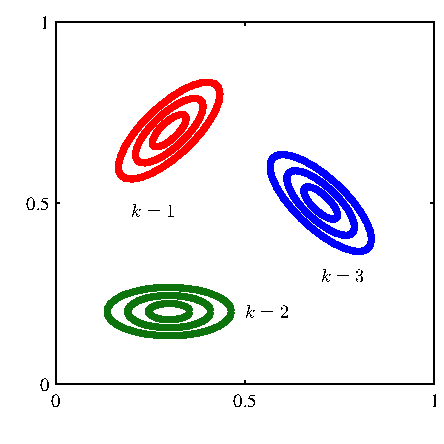
\includegraphics[width = .5\textwidth, transparent]{figs/Figure13_8a}
%			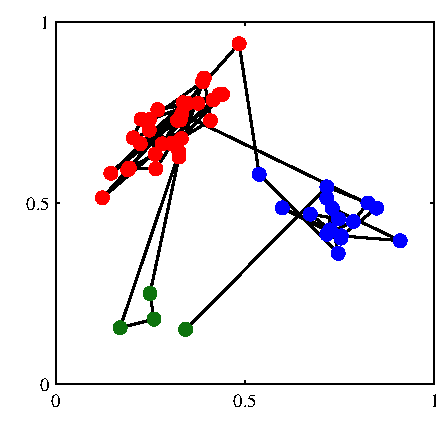
\includegraphics[width = .5\textwidth, transparent]{figs/Figure13_8b}
%		\end{center}
%	\end{figure}
%	Visualization from PRML. \citep{Bishop06}
%
%}

%\frame[t] {
%\frametitle{ HMM: Trellis}
% \begin{figure}[t]
%		\begin{center}
%			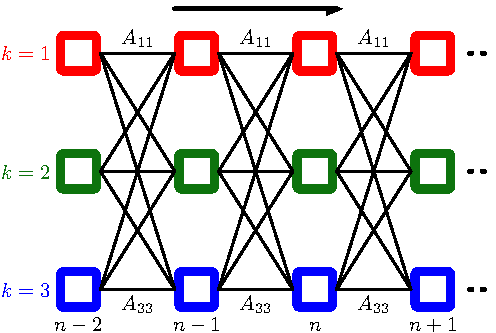
\includegraphics[width = .7\textwidth, transparent]{figs/Figure13_7}
%		\end{center}
%	\end{figure}
%	Visualization from PRML. \citep{Bishop06}
%
%}


\frame[t] {
\frametitle{HMM: Typical Usage Scenario (Character Recognition)}
\begin{itemize}
\item Training data: multiple ``observed''  $y_t = \{v_t,h_t\}$ sequences of stylus positions for each kind of character %(stroke boundaries unobserved but important ``structurally'' --- correspond to latent states)
\item Task: train $|\Sigma|$ different models, one for each character %(Maximum likelihood training via EM: {\em Baum-Welch} \citep{baum1972equality}, {\em forward-backward} \citep{Rabiner:1989}, belief propagation \citep{Bishop06})
\item Latent states: sequences of strokes 
\item Usage: classify new stylus position sequences using trained models  $\mathcal{M}_\sigma = \{A_\sigma, \Theta_\sigma\}$% and Bayes factors
\[ P(  \mathcal{M}_\sigma | y_1,\ldots,y_T) \propto P(y_1,\ldots,y_T | \mathcal{M}_\sigma) P( \mathcal{M}_\sigma) \]
 %which requires marginalizing out $z$'s 
%\[ P(y_1,\ldots,y_T | \mathcal{M}_\sigma) = \sum_Z P(y_1,\ldots,y_T, z_0, \ldots, z_T | A_\sigma, \Theta_\sigma)\]
\end{itemize}

}

\frame[t] {
\frametitle{Shortcomings of Original HMM Specification}
\begin{itemize}
\item Latent state dwell times are not usually geometrically distributed
\eqan
\lefteqn{P(z_{t} = m, \ldots, z_{t+L} = m | A)} \nonumber \\
 &=& \prod_{\ell = 1}^L P(z_{t+\ell+1} = m| z_{t+\ell} = m, A) \nonumber \\
 &=& \mathsf{Geometric}(L; \bsym\pi_m(m)) \nonumber
 \enan
\item Prior knowledge often suggests structural constraints on allowable transitions
\item The state cardinality of the latent Markov chain $K$ is usually unknown
\end{itemize}

}

\section{Related Work}

\frame[t] {
\frametitle{Explicit Duration HMM / H. Semi-Markov Model}
\citep{Mitchell95,Murphy02,Yu03,Yu:2010}
\begin{itemize}
\item Latent state sequence $\bsym z = (\{s_{1},r_1\},\dots, \{s_{T},r_T\})$
\item Latent state id sequence $\bsym s = (s_{1},\dots, s_{T})$
\item Latent ``remaining duration'' sequence $\bsym r = (r_{1},\dots, r_{T})$
%\item Observation sequence $\bsym y = (y_{1}, \dots, y_{T})$
\item State-specific duration distribution $F_{r}(\lambda_{m})$
%\item State transition matrix with columns $\bsym \pi_{m} = (\pi_{m1},\pi_{m2},\dots, \pi_{mM})$
%\item State-specific observation distribution $y_{t} \sim F_{\theta}(\theta_{m})$
\item Other distributions the same
\end{itemize}

An EDHMM transitions between states in a different way than does a typical HMM. Unless $r_{t} = 0$  the current remaining duration is decremented and the state does not change.  If $r_{t} = 0$ then the EDHMM transitions to a state $m \ne s_{t}$ according to the distribution defined by $\bsym \pi_{s_{t}}$ \newline

Problem: inference requires enumerating possible durations.

%A finite explicit duration HMM (EDHMM) consists of a hidden state sequence $\bsym s = (s_{1},\dots, s_{T})$, the corresponding observation sequence $\bsym y = (y_{1}, \dots, y_{T})$, and a latent ``remaining duration'' sequence $\bsym r = (r_{1},\dots, r_{T})$.  It also has a state transition matrix  $\bsym \pi$, where the row vector $\bsym \pi_{m} = (\pi_{m1},\pi_{m2},\dots, \pi_{mM})$ corresponds to the transition probabilities out of state $m$, and $\bsym \pi_{0}$ is the initial state vector. An EDHMM transitions between states in a different way than does a typical HMM. Unless $r_{t} = 0$  the current remaining duration is decremented and the state does not change.  If $r_{t} = 0$ then the EDHMM transitions to a state $m \ne s_{t}$ according to the distribution defined by $\bsym \pi_{s_{t}}$. The duration the HMM will remain in the new state $m$ is drawn from the  state-specific duration distribution $F_{r}(\lambda_{m})$ governed by parameter $\lambda_{m}$. At each timestep the observation $y_{t} \sim F_{\theta}(\theta_{m})$ is drawn from a state-specific emission distribution parameterized by $\theta_{m}$.   The emission distribution parameters are given a shared prior $\theta_m \sim H_{\theta}$. The EDHMM is an EDHMM with a countable number of states, i.e.~$M\rightarrow\infty$.


}

\frame[t] {
\frametitle{EDHMM notation}

Latent state $z_t = \{s_t, r_t\}$ is tuple consisting of state identity and time left in state.

\eqan
%\theta_{m} &\sim& H_{\theta} \nonumber \\
%\lambda_{m} &\sim& H_{r}\nonumber \\
\!\!\!\!\! s_{t} | s_{t-1}, r_{t-1} &\sim& 
	\begin{cases} 
	\mathbb I(s_{t} = s_{t-1}), & \! r_{t-1} > 0 \\
	\mathsf{Discrete}(\bsym\pi_{s_{t-1}}), & r_{t-1} = 0
	\end{cases}\nonumber \\
\!\!\!\!\! r_{t } | s_{t}, r_{t-1} &\sim& 
	\begin{cases} 
	\mathbb I(r_{t} = r_{t-1} - 1),& r_{t-1} > 0 \\
	F_{r}(\lambda_{s_{t}}),& r_{t-1} = 0
	\end{cases} \nonumber\\
y_{t} | s_{t} &\sim& F_{\theta}(\theta_{s_{t}})\nonumber
\enan


}

\frame[t] {
\frametitle{EDHMM: Graphical Model}
\begin{figure}[t]
		\begin{center}
			\includegraphics[width = \textwidth, transparent]{figs/EDHMM-graphical-model}
		\end{center}
	\end{figure}
}





\frame[t] {
\frametitle{Structured HMMs: i.e.~left-to-right HMM \citep{Rabiner:1989}}

\begin{block}{Example: Chicken pox}
\begin{description}
\item[Observations] vital signs
\item[Latent states] pre-infection, infected, post-infection\footnote{disregarding shingles} 
\item[State transition structure]  can't go from infected to pre-infection
\end{description}
\end{block}
Structured transitions also imply zeros in the transition matrix $A$, i.e.

\[p(s_t = m | s_{t-1} = \ell) = 0 \; \forall \; m < \ell\]


}


%\frame[t] {
%\frametitle{Structured HMM: Trellis: One step at a time, left-to-right HMM }
%
% \begin{figure}[t]
%		\begin{center}
%			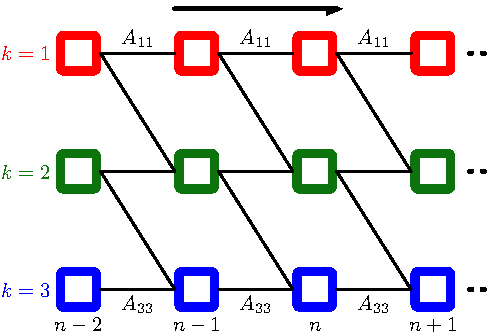
\includegraphics[width = .7\textwidth, transparent]{figs/Figure13_10}
%		\end{center}
%	\end{figure}
%	Figure from PRML. \citep{Bishop06}
%
%}

\frame[t] {
\frametitle{Bayesian HMM}

\begin{itemize}
\item We will put a {\em prior} on parameters so that we can effect a solution that conforms to our  ideas about what the solution should look like 

\begin{itemize}
\item Structured prior examples
\begin{itemize}
\item $A_{i,j}=0$ (hard constraints)
\item $A_{i,j}\approx \sum_j A_{i,j}$ (rich get richer)
\end{itemize}
\end{itemize}


\item  {\em Regularization} means that we can specify a model with more parameters than could possibly be needed
\begin{itemize}
\item infinite complexity  (i.e.~$K \rightarrow \infty$) avoids many model selection problems
\item  ``extra'' states can be thought of as auxiliary or nuisance variables 
\item inference requires sampling in a model with countably infinite support
\end{itemize}
%\item  Posterior inference treats parameters $A$ and $\Theta$ as latent variables
\item Posterior over latent variables encodes uncertainty about interpretation of data.
\end{itemize}


}

%\frame[t] {
%\frametitle{Bayesian HMM}
% Posterior inference treats parameters as latent variables and marginalizes them out too. \newline
%
%%Consider the earlier sequence classification task, now
%
%%\[P(\{y_1,\ldots,y_T\}^{\mbox{new}} |  \]
%%
%%\[ P(  \mathcal{M}_\sigma | y_1,\ldots,y_T) \propto P(y_1,\ldots,y_T | \mathcal{M}_\sigma) P( \mathcal{M}_\sigma) \]
%% which requires marginalizing out $z$'s {\em and} $A$ and $\Theta$
%%\eqan
%%\lefteqn{P(y_1,\ldots,y_T | \mathcal{H})}\nonumber \\
%%&=& \int \int \sum_Z P(y_1,\ldots,y_T, z_0, \ldots, z_T,  A_\sigma, \Theta_\sigma| \mathcal{H}) dP(A_\sigma) dP(\Theta_\sigma)
%%\enan
%%where $\mathcal{H}$ is a set of hyperparameters.
%
%
%
%}

\frame[t] {
\frametitle{Bayesian HMM}
\begin{figure}[t]
		\begin{center}
			\includegraphics[width = \textwidth, transparent]{figs/Bayesian-HMM-graphical-model}
		\end{center}
	\end{figure}
%
\alert<1>{\eqan
\bsym\pi_{m} &\sim& H_{z} \nonumber \\
\theta_{m} &\sim& H_{y} \nonumber 
\enan}%
\eqan
\!\!\!\!\! z_{t} | z_{t-1}=m &\sim&
	\mathsf{Discrete}(\bsym\pi_{m})
	\nonumber \\
y_{t} | z_{t}=m &\sim& F_{\theta}(\theta_{m})\nonumber
\enan
}


\frame[t] {
\frametitle{Infinite HMMs (IHMM) \citep{Beal:2002,Teh:2006b}}
 
 
 
 \begin{figure}[t]
		\begin{center}
			\includegraphics[width = \textwidth, transparent]{figs/iHMM-graphical-model}
		\end{center}
	\end{figure}
	  \[K \rightarrow \infty, \]
	  Sticky Infinite HMM \citep{Fox:2010tg}


}
%
%\frame[t] {
%\frametitle{Other HMM variants}
%\begin{itemize}
%\item Sticky Infinite HMMs \citep{Fox:2010tg}
%\begin{itemize}
%\item Extra parameter per state used to bias towards self-transition
%\end{itemize}
%\item Hierarchical HMMs \citep{Murphy01a} 
%\begin{itemize}
%\item State is hierarchical (i.e.~sequence of letters composed of stroke sequences)
%\end{itemize}
%\item  Factorial HMMs \citep{Ghahramani96a}
%%\begin{itemize}
%%\item State is binary encoding 
%%\end{itemize}
%\item  Infinite explicit duration HMM \citep{Johnson:2010}
%\begin{itemize}
%\item No generative model. Latent history sampling used to assert the existence of an implicitly defined EDHMM that can be sampled from by rejecting HDP-HMM samples that violate transition constraints.
%\end{itemize}
%\end{itemize}
%
%}

\frame[t] {
\frametitle{Inference for the Explicit Duration HMM (EDHMM) }

Simple Idea
\begin{itemize}
\item Infinite HMMs and EDHMMs share fundamental characteristic: countable support
\item Inference techniques for Bayesian nonparametric (infinite) HMMs can be used for EDHMM inference
\end{itemize}
Result
\begin{itemize}
\item Approximation-free, efficient inference algorithm for EDHMM inference
%\begin{itemize}
%\item Example: explicit duration HMM's require no self-transitions \[\bsym\pi_i(i)=A_{i,i}=0\]
%\item HDP-HMM construction good for dependence, doesn't work for structure
%\end{itemize}
%The HDP-HMM construction of the iHMM  \citep{Teh:2006b, VanGael:2008} would seem to be a good way to construct an EDHMM. 
%In sich a construction each row of $\bsym\pi$ (of which there a countably infinite number) would be a draw from a Dirichlet process (DP) with base measure $D_{0} = \sum_{k=1}^{\infty} w_{k}\delta_{\theta_{k}}$, where $D_{0}$ is itself a draw from a Dirichlet process with base measure $H_{\theta}$.
%Therefore, the $m$-th draw $D_{m} \sim \textnormal{DP}(c_{0}D_{0})$ can be written as $D_{m} = \sum_{k} \pi_{mk}\delta_{\theta_{k}}$. 
%Unfortunately the EDHMM cannot be constructed in this manner because the HPD-HMM cannot enforce the kind of dependence required by the no self-transition condition $m \ne s_{t}$.  This is because the HDP prior on the transition distributions requires that any time a state is transitioned to from any other state it becomes more likely to be transitioned to by all other states.  Unfortunately developing a a model in which the state transition distributions exhibit dependence on a covariate or auxiliary variable requires the abandoning the conditional independence requirement of the HDP.
%\item How to do inference in HMMs with countable state cardinality and countable duration distribution support.
\end{itemize}
%\;\;\;\;\;\;\citepalias{Huggins-2012-AISTATS}
}

\begin{frame}[t]{Bayesian EDHMM: Graphical Model}
	\begin{figure}[t]
		\begin{center}
			\includegraphics[height = 4cm, transparent]{figs/Bayesian-EDHMM-graphical-model}
		\end{center}
	\end{figure}
A choice of prior
\begin{eqnarray*}
\lambda_m | H_r &\sim&  \mathsf{Gamma}(H_r)\\
\pi_m | H_z &\sim& \mathsf{Dir}(1/K, 1/K, \ldots,  1/K, 0,1/K, \ldots,  1/K,  1/K) \\
\end{eqnarray*}


\end{frame}
%
%\frame[t] {
%\frametitle{EDHMM: Recipe}
%\begin{itemize}
%\item Poisson process \citep{Kingman:1993} 
%\item Gamma process \citep{Kingman:1993} 
%\item SN\GP s \citep{Rao:2009}
%\item {\em Structured, dependent, infinite-dimensional} transition distributions \citepalias{Huggins-2012-AISTATS}
%\end{itemize}
%
%}
%
%\frame[t] {
%\frametitle{EDHMM: Recipe}
%
%\begin{itemize}
%\item Gamma process  \citep{Kingman:1993} as Poisson process over $\Theta \otimes V \otimes [0,\infty)$ with rate / mean measure
%\eqn \mu(\tilde\Theta, \tilde V,  \tilde S) = \alpha(\tilde\Theta, \tilde V) \int_{\tilde S}\gamma^{-1}e^{-\gamma} \nonumber \enn
%\item A draw from a Gamma process with \[\alpha(\tilde\Theta,  \tilde V) = c_{0}H_{\theta}(\tilde\Theta)H_{v}( \tilde V).\] \citep{Kingman:1993} has the form
%\eqn G  = \sum_{m=1}^{\infty} \gamma_{m} \delta_{(\theta_{m}, v_{m})} \nonumber \enn
%where $(\theta_{m}, v_{m}) \sim H_{\theta}\times H_{v}$. \newline
%\end{itemize}
%
%}
%\frame[t] {
%\frametitle{EDHMM: Recipe}
%\begin{itemize}
%\item Non-disjoint ``restricted projections'' of Gamma processes are {\em dependent} Gamma processes (SN\GP s) \citep{Rao:2009}
%\begin{figure}[t]
%		\begin{center}
%			\includegraphics[width=.75\textwidth, transparent]{figs/isedhmm_geom_base_gp}
%		\end{center}
%	\end{figure}
%	
%	\end{itemize}
%
%\eqn G_0 = \sum_{m\neq0} \ldots, \;\;\;\cdots\;\;\;,G_4  = \sum_{m\neq4} \gamma_{m} \delta_{\theta_{m}},\;\;\;\cdots\;\;\;  \nonumber \enn
%
%}
%	
%	
%\frame[t] {
%\frametitle{EDHMM: Recipe}
%
%	\begin{itemize}
%
%\item Normalized dependent \GP~draws are dependent Dirichlet process draws.\footnote{a draw from a Dirichlet process \citep{Ferguson1973} is an infinite sum of weighted atoms \citep{Sethuraman1994} where the weights sum to one.}  In the EDHMM, DP draws are the dependent, structured, infinite-dimensional transition distributions
%
%\eqan D_4  &=& \frac{G_4}{G_4(\Theta)} \\
% &=& \frac{\sum_{m\neq4} \gamma_{m} \delta_{\theta_{m}}}{\sum_{\theta \in \Theta}\sum_{m'\neq4} \gamma_{m'} \delta_{\theta_{m'}}} \\
% &=& \frac{\sum_{m\neq4} \gamma_{m} \delta_{\theta_{m}}}{\sum_{m'\neq4} \gamma_{m'}}\\
% &=& \sum_{m\neq4} \frac{\gamma_{m}}{\sum_{m'\neq4} \gamma_{m'}} \delta_{\theta_{m}} \nonumber \enan
%	\end{itemize}
%
%}
%
%\frame[t] {
%\frametitle{EDHMM: Recipe}
%	\begin{figure}[t]
%		\begin{center}
%			\includegraphics[height = 6cm, transparent]{figs/ED-iHMM-hierarchical-model}
%		\end{center}
%	\end{figure}
%	
%	\begin{itemize}
%
%\item Structured, dependent, infinite dimensional transition distributions $\bsym\pi_m$ can be formed from draws from DDPs \citepalias{Huggins-2012-AISTATS}
%%\item Auxiliary variables
%%\item Beam Sampling
%\end{itemize}
%}

%\begin{frame}[t]{EDHMM: Geometric base distribution over states example}
%	\end{frame}

%\frame[t] {
%\frametitle{Structured Transitions Via Dependent Dirichlet Processes}
%\begin{itemize}
%\item<1-3> One way to define a set of dependent DPs is to construct a base gamma process over an augmented space by taking the union of disjoint independent gamma processes, then define a series of restricted projections of that base process, which are themselves gamma processes. 
%
%\item<2-3> The normalization of these dependent gamma processes form a set of dependent DPs.  
%
%\item<3-3> We will use this procedure to construct a number of dependent DPs (one for each HMM state) which preclude certain transitions.  The precluded transitions, a form of dependence,  arise from particulars.
%\end{itemize}
%
%}


\frame[t] {
\frametitle{EDHMM Inference: Beam Sampling  \citepalias{Dewar:2011}}
We employ the forward-filtering, backward slice-sampling approach for the IHMM of \citep{VanGael:2008} , %This so-called beam sampling approach is an auxiliary variable slice-sampling approach. 
in which the state and duration variables $\bsym s$ and $\bsym r$ are sampled conditioned on auxiliary slice variables $\bsym u$. \newline % via a forward-chainin 

Net result: efficient, always finite forward-backward procedure for sampling latent states and the amount of time spent in them.

}



\frame[t] {
\frametitle{Auxiliary Variables for Sampling}
\begin{columns}[t]
\begin{column}{.5\textwidth}

Objective: get samples of $x$.  \newline 

\uncover<2->{Sometimes it is easier to introduce an auxiliary variable $u$ and to Gibbs sample the joint $P(x,u)$ (i.e.~sample from $P(x|u; \lambda)$ then $P(u|x, \lambda)$, etc.) then discard the $u$ values than it is to directly sample from $p(x|\lambda)$. \newline}%

\uncover<3->{Useful when: $p(x|\lambda)$ does not have a known parametric form but adding $u$ results in a parametric form {\em and} when $x$ has countable support and sampling it requires enumerating all values. }

	\end{column}
	\begin{column}{.25\textwidth}
\uncover<1->{\begin{figure}[t]
		\begin{center}
			\includegraphics[height = 3cm, transparent]{figs/poisson_slice_sampling_example_before_aux}
		\end{center}
	\end{figure}
	}
	\end{column}
		\begin{column}{.25\textwidth}

	\uncover<2->{\begin{figure}[t]
		\begin{center}
			\includegraphics[height = 5cm, transparent]{figs/poisson_slice_sampling_example}
		\end{center}
	\end{figure}
	}
	\end{column}
	\end{columns}


}




\frame[t] {
\frametitle{Slice Sampling: A {\em very} useful auxiliary variable sampling trick}
Pedagogical Example: 
\begin{itemize}
\item $x|\lambda \sim \mathsf{Poisson}(\lambda)$ (countable support)
\item  {\em enumeration} strategy for sampling $x$ (impossible)\footnote{Necessary in EDHMM}
\item auxiliary variable $u$ with $P(u|x,\lambda) = \frac{\mathbb{I}(0 \leq u \leq P(x|\lambda))}{P(x|\lambda)}$
\end{itemize}
Note:
Marginal distribution of $x$ is 
\eqan
P(x|\lambda) &=& \sum_u P(x,u|\lambda) \nonumber\\
&=& \sum_u P(x|\lambda)P(u|x,\lambda) \nonumber\\
&=& \sum_u P(x|\lambda) \frac{\mathbb{I}(0 \leq u \leq P(x|\lambda))}{P(x|\lambda)}\nonumber\\
&=& \sum_u \mathbb{I}(0 \leq u \leq P(x|\lambda)) = P(x|\lambda) \nonumber
\enan

}

\frame[t] {
\frametitle{Slice Sampling: A {\em very} useful auxiliary variable sampling trick}
This suggests a Gibbs sampling scheme: alternately sampling from
\begin{itemize}
\item $P(x|u,\lambda) \propto \mathbb{I}(u \leq P(x|\lambda))$ 
\begin{itemize}
\item {\em finite} support, uniform above slice, enumeration {\em possible}
\end{itemize}
\item  $P(u|x,\lambda) = \frac{\mathbb{I}(0 \leq u \leq P(x|\lambda))}{P(x|\lambda)}$ 
\begin{itemize}
\item uniform between 0 and $y=P(x|\lambda)$
\end{itemize}
\end{itemize}
then discarding the $u$ values to arrive at $x$ samples marginally distributed according to $P(x|\lambda)$.
\begin{figure}[t]
		\begin{center}
			\includegraphics[width = .6\textwidth, transparent, trim=3cm 8cm 3cm 9cm, clip]{figs/poiss_pdf_slice}
		\end{center}
	\end{figure}

}

\frame[t] {
\frametitle{EDHMM Graphical Model with Auxiliary Variables}
\begin{figure}[t]
		\begin{center}
			\includegraphics[width = .85\textwidth, transparent]{figs/EDHMM-graphical-model-with-aux-vars.pdf}
		\end{center}
	\end{figure}
}


\frame[t] {
\frametitle{EDHMM Inference: Beam Sampling}
With auxiliary variables defined as

\eqn p(u_{t} | z_{t}, z_{t-1}) = \frac{\mathbb I(0 < u_{t} < p(z_{t} | z_{t-1}))}{ p(z_{t} | z_{t-1})} \nonumber \enn

and

\eqan
 p(z_{t} | z_{t-1}) &=&
 p((s_t , r_t ) | (s_{t-1}, r_{t-1}))  \nonumber \\
	&=&\begin{cases} 
	r_{t-1} > 0, & \mathbb{I}(s_t=s_{t-1})\mathbb{I}(r_t = r_{t-1}-1) \\
	r_{t-1} = 0, & \pi_{s_{t-1}s_{t}}F_r(r_t;\lambda_{s_t}).
	\end{cases} \nonumber 
\enan

one can run standard forward-backward conditioned on $u$'s.\newline

Forward-backward slice sampling only has to consider a finite number of successor states at each timestep.  
}

\frame[t] {
\frametitle{Forward recursion}
\begin{eqnarray}
   \hat{\alpha}_t(z_t) &=& 
   p(z_t, \mathcal{Y}_1^t , \mathcal{U}_1^{t})   \nonumber \\
   &=& 
   \sum_{z_{t-1}}
   p(z_t, z_{t-1} , \mathcal{Y}_1^t , \mathcal{U}_1^{t}) \nonumber \\
   &\propto& 
   \sum_{z_{t-1}}
   p(u_{t} | z_t, z_{t-1})
   p(z_t, z_{t-1} , \mathcal{Y}_1^t, \mathcal{U}_1^{t-1}) \nonumber \\
   &=& 
   \sum_{z_{t-1}}
   \mathbb{I}(0 < u_{t} < p(z_t | z_{t-1}))
   p(y_t|z_t) \hat{\alpha}_{t-1}(z_{t-1}) \nonumber.
\end{eqnarray}

}

\frame[t] {
\frametitle{Backward Sampling}
Recursively sample a state sequence from the distribution $p(z_{t-1} | z_{t}, \mathcal{Y}, \mathcal{U})$
%\begin{equation}
%    p(z_t | z_{t+1}, \mathcal{Y}, \mathcal{U}).
%\end{equation}
which can expressed in terms of the forward variable:
\begin{eqnarray}
    p(z_{t-1} | z_{t}, \mathcal{Y}, \mathcal{U}) &\propto& p(z_{t},z_{t-1}, \mathcal{Y}, \mathcal{U})  \label{eqn:backward} \nonumber \\
    & \propto &  
        p(u_{t} | z_t, z_{t-1})p(z_{t}|z_{t-1}) \hat{\alpha}_{t-1}(z_{t-1})
        %p(z_t, \mathcal{Y}_1^t, \mathcal{U}_1^t)
        %p(\mathcal{Y}_{t+1}^T, \mathcal{U}_{t+2}^T | z_{t+1}) 
        \nonumber\\
    & \propto & 
       \mathbb{I}(0 < u_{t} < p(z_{t} | z_{t-1}))
        \hat{\alpha}_{t-1}(z_{t-1}).\nonumber
\end{eqnarray}

}


\frame[t] {
\frametitle{Results}
To illustrate EDHMM learning on synthetic data, five hundred datapoints were generated using a 4 state EDHMM with Poisson duration distributions \[\bsym \lambda = (10, 20, 3, 7)\] and Gaussian emission distributions with means \[\bsym \mu = (-6, -2, 2, 6)\] all unit variance. 
}

\begin{frame}[t]{EDHMM: Synthetic Data Results}
	\begin{figure}[t]
		\begin{center}
			\includegraphics[height = 7cm, transparent]{figs/state-distribution-figure}
		\end{center}
	\end{figure}
\end{frame}

\begin{frame}[t]{EDHMM: Synthetic Data, State Mean Posterior}
	\begin{figure}[t]
		\begin{center}
			\includegraphics[height = 6cm, transparent]{figs/4-states-4-apart-1-variance-mean-posteriors-big-font}
		\end{center}
	\end{figure}
\end{frame}

\begin{frame}[t]{EDHMM: Synthetic Data, State Duration Parameter Posterior }
	\begin{figure}[t]
		\begin{center}
			\includegraphics[height = 6cm, transparent]{figs/4-states-4-apart-1-variance-duration-posteriors-big-font}
		\end{center}
	\end{figure}
\end{frame}



\begin{frame}[t]{EDHMM: Nanoscale Transistor Spontaneous Voltage Fluctuation}
	\begin{figure}[t]
		\begin{center}
			\includegraphics[height = 6cm, transparent]{figs/RTS-ED-iHMM-overlay}
		\end{center}
	\end{figure}
\end{frame}





\begin{frame}[t]{EDHMM:  States Not Distinguishable By Output}
Task: understand system with states that have identical observation distributions and differ only in  duration distribution. \newline

Observation distributions have means $\mu_1 = 0$, $\mu_2 = 0$, and $\mu_3 = 3$ and the duration distributions have rates $\lambda_1 = 5$, $\lambda_2 = 15$, $\lambda_3 = 20$. \newline 

(Next slide) \newline 

a) observations; b) true states overlaid with 20 randomly selected state traces produced by the sampler.  \newline

Samples from the posterior observation distribution mean are shown in c), and samples from the posterior duration distribution rates are shown in d).
\end{frame}

\begin{frame}[t]{EDHMM:  States Not Distinguishable By Output}
\setcounter{subfigure}{0}
\begin{figure}
    \subfigure[][]{
        \includegraphics[width=0.9\textwidth]{pic/experiment_3_Y.pdf}
        \label{fig:exp_2_data}
    } \\
    \subfigure[][]{
        \includegraphics[width=0.9\textwidth]{pic/experiment_3_X.pdf}
        \label{fig:exp_2_state}
    } \\
    \subfigure[][]{
        \includegraphics[width=0.45\textwidth]{pic/posterior_means_exp3.pdf}
        \label{fig:posterior_means_3}
    } 
    \subfigure[][]{
        \includegraphics[width=0.45\textwidth]{pic/posterior_rates_exp3.pdf}
        \label{fig:posterior_rates_3}
    }
    \caption{Beam sampler results applied to a system with identical observation distributions but differing durations. Observations are shown in a); true states are shown in b) overlaid with 20 randomly selected state traces produced by the sampler. Here the observation distributions have means $\mu_1 = 0$, $\mu_2 = 0$, and $\mu_3 = 3$ and the duration distributions have rates $\lambda_1 = 5$, $\lambda_2 = 15$, $\lambda_3 = 20$. Samples from the posterior observation distribution mean are shown in c), and samples from the posterior duration distribution rates are shown in d).}
    \label{fig:experiment2_results}
\end{figure}
\end{frame}

\begin{frame}[t]{EDHMM vs. IHMM:  Modeling the Morse Code Cepstrum}
	\begin{figure}[t]
		\begin{center}
			\includegraphics[height = 6cm, transparent]{figs/morse-spectrogram-ED-iHMM-and-iHMM-output}
		\end{center}
	\end{figure}
\end{frame}

\begin{frame}[t]{Wrap-Up}
\begin{itemize}
\item Novel inference procedure for EDHMMs that doesn't require truncation and is more efficient than considering all possible durations.
\end{itemize}
\begin{figure}
    \includegraphics[width=0.85\textwidth]{pic/number_transitions_visited.pdf}

\caption{Mean number of transitions considered per time point by the beam sampler for 1000 post-burn-in iterations. Compare to $(KT)^2 = O(10^6)$ transitions that would need to be considered by standard forward backward without truncation, the only surely safe, truncation-free alternative.}
\label{fig:allowed}
\end{figure}

\end{frame}

\begin{frame}[t]{Future Work}
\begin{itemize}
\item Novel Gamma process construction for dependent, structured, infinite dimensional HMM transition distributions.
%\item Other transition distribution structures (left-to-right) can be implemented simply by changing ``restricted projection regions.''
%\item EDHMM framework generalizes the HMM, Bayesian HMM, infinite HMM, left-to-right HMM, explicit duration HMM, and more.
\item Generalize to spatial prior on HMM states (``location'')
\begin{itemize}
\item Simultaneous location and mapping
\item Process diagram modeling for systems biology
\end{itemize}
\item Applications; seeking ``users''
\end{itemize}

\end{frame}

\begin{frame}[t]{Questions?}

Thank you!

\end{frame}



	\bibliographystyle{plainnat}
	\begin{frame}[t,allowframebreaks]{Bibliography}

\bibliography{../../papers/uber}
\end{frame}



\end{document}
